\documentclass[11pt, a4paper]{article}

% ----- Packages -----
\usepackage[utf8]{inputenc}
\usepackage{amsmath, amssymb}
\usepackage{geometry}
\geometry{top=1in, bottom=1in, left=1in, right=1in}
\usepackage{float}
\usepackage{tikz}
\usetikzlibrary{arrows.meta, positioning}

% ----- Advanced TikZ Styles -----
\tikzset{
    feNode/.style={
        circle, 
        draw=black, 
        fill=white, 
        thick, 
        inner sep=0pt, 
        minimum size=1.8mm
    }
}

\begin{document}

% ----- Header -----
\begin{center}
    {\Large \textbf{Homework 1}} \\[0.2cm]
    {\large \textbf{CE 512 Finite Element Method}} \\[0.1cm]
    {\large 2026 Spring} \\[0.3cm]
    \textbf{Due Date:} 02.03.2026-01:00 (upload to \texttt{https://cloud-lms.iyte.edu.tr})
\end{center}

\vspace{0.5cm}

% ----- Introduction -----
\noindent The following problems are based on the class notes, but they are modified in order to improve your understanding of the phenomenology. \\

\noindent \textbf{Derive the following problems without making any shortcuts.}

\vspace{0.5cm}

% ----- Problems -----
\begin{enumerate}
    
    % Problem 1
    \item By using the phenomenology presented in class, derive the stiffness matrix for the following truss member. Note that the degrees of freedom are positive when pointing out of the element.
    
    \begin{figure}[H]
        \centering
        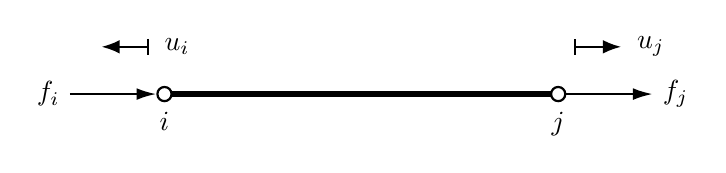
\begin{tikzpicture}[>={Latex[length=2.5mm, width=1.5mm]}]
            % Coordinates
            \coordinate (i) at (0,0);
            \coordinate (j) at (5,0);
            
            % Element Line
            \draw[line width=2pt] (i) -- (j);
            
            % Nodes
            \node[feNode, label=below:{$i$}] (NodeI) at (i) {};
            \node[feNode, label=below:{$j$}] (NodeJ) at (j) {};
            
            % Force arrows (f)
            \draw[->, thick] (-1.2,0) -- (NodeI) node[pos=0, left] {$f_i$};
            \draw[->, thick] (NodeJ) -- (6.2,0) node[pos=1, right] {$f_j$};
            
            % Displacement arrows (u) with vertical bar tails
            \draw[{Latex}-{Bar[width=2mm]}, thick] (-0.8, 0.6) -- (-0.2, 0.6) node[pos=1, right=2pt] {$u_i$};
            \draw[{Bar[width=2mm]}-{Latex}, thick] (5.2, 0.6) -- (5.8, 0.6) node[pos=1, right=2pt] {$u_j$};
        \end{tikzpicture}
    \end{figure}

    \vspace{0.2cm}

    % Problem 2
    \item Similar to Pr.1, derive the ``cold'' conduction formula for the following configuration. 
    \[ q^{c} = \frac{\text{cold flux}}{\text{area}} \]
    and $q > 0$ when directed out of the element. $-q^{c}$ flows from low temperature to high temperature.
    
    \begin{figure}[H]
        \centering
        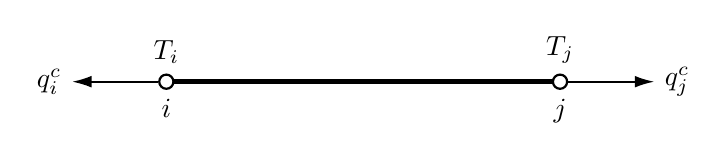
\begin{tikzpicture}[>={Latex[length=2.5mm, width=1.5mm]}]
            % Coordinates
            \coordinate (i) at (0,0);
            \coordinate (j) at (5,0);
            
            % Element Line
            \draw[line width=2pt] (i) -- (j);
            
            % Nodes
            \node[feNode, label=below:{$i$}, label=above:{$T_i$}] (NodeI) at (i) {};
            \node[feNode, label=below:{$j$}, label=above:{$T_j$}] (NodeJ) at (j) {};
            
            % Flux arrows (q^c)
            \draw[->, thick] (NodeI) -- (-1.2,0) node[pos=1, left] {$q_i^c$};
            \draw[->, thick] (NodeJ) -- (6.2,0) node[pos=1, right] {$q_j^c$};
        \end{tikzpicture}
    \end{figure}

    \vspace{0.2cm}

    % Problem 3
    \item Similar to Pr.1, derive the current conduction matrix for the following resistive wire segment.
    
    \begin{figure}[H]
        \centering
        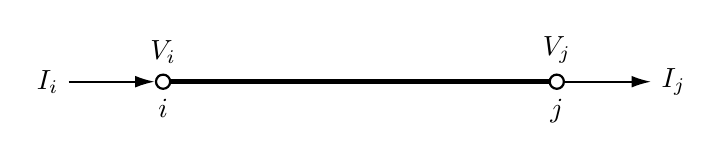
\begin{tikzpicture}[>={Latex[length=2.5mm, width=1.5mm]}]
            % Coordinates
            \coordinate (i) at (0,0);
            \coordinate (j) at (5,0);
            
            % Element Line
            \draw[line width=2pt] (i) -- (j);
            
            % Nodes
            \node[feNode, label=below:{$i$}, label=above:{$V_i$}] (NodeI) at (i) {};
            \node[feNode, label=below:{$j$}, label=above:{$V_j$}] (NodeJ) at (j) {};
            
            % Current arrows (I)
            \draw[->, thick] (-1.2,0) -- (NodeI) node[pos=0, left] {$I_i$};
            \draw[->, thick] (NodeJ) -- (6.2,0) node[pos=1, right] {$I_j$};
        \end{tikzpicture}
    \end{figure}

\end{enumerate}

\end{document}